\section{Instruction set architecture}
The goal for the beggining of this course is to go from "high-level" perspective to the bottom of the iceberg. First let us look at a piece of code (\texttt{c}):

\begin{lstlisting}[language=c]
int data = 0x00123456;
int result = 0;
int mask = 1;
int count = 0;
int temp = 0;
int limit = 32;
do{
   temp = data & mask;
   result = result + temp;
   data = data >> 1;
   count = count + 1;
} while (count != limite);
\end{lstlisting}
Here we can see that we have variable with expressive names (that we can choose). each variable has a type, the computation we are doing \texttt{result + temp} looks like a mathematic formula, the control flow we are using is very intuitive.\\
In the case of those high-level language, we have an "unlimited" number of variables which supports any type.\\
If we wanted to convert this code into Assembly code we would have this:
\begin{lstlisting}[language={[RISC-V]Assembler}]
    li x1, 0x00123456
	li x2, 0 
	li x3, 1 
	li x4, 0 
	li x5, 0 
	li x6, 32
loop:
	and x5, x1, x3
	add x2, x2, x5 
	srli x1, x1, 1 
	addi x4, x4, 1 
	bne x4, x6, loop
\end{lstlisting}
As we can see we have a much more rigid format: we really have a sequence of numbered instructions that is executed line by line. For each instructions, we have an \textit{opcode}  that defines the effect of the instruction. Each \textit{variable} has a fixed name and we only have one form of control flow. The question to ask is why did we do that?\\ The answer of thie question lays is in the architecture of the processor:
\begin{center}
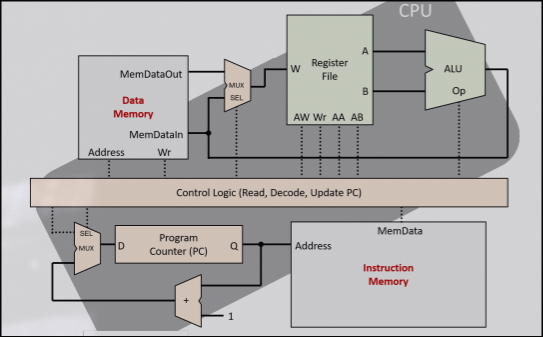
\includegraphics[scale=0.6]{screenshots/2025-10-11_1.png}
\end{center}
how it works: the processor fetch the instruction at the address of the program counter (PC) and launch it to the control logic
\begin{center}
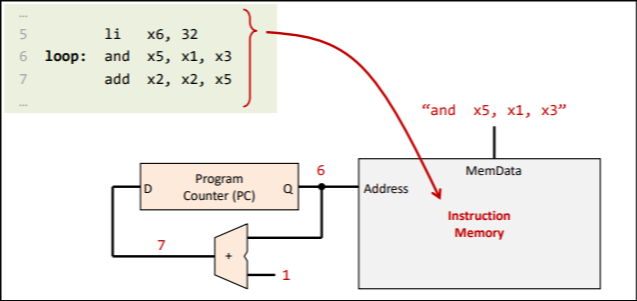
\includegraphics[scale=0.6]{screenshots/2025-10-11_2.png}
\end{center}
After that the instruction has been fetch, it is processed in the Control logic and then read/write etc... into the register file, and give the information (the opcode) to the ALU for it to know which operation to perform.
\begin{center}
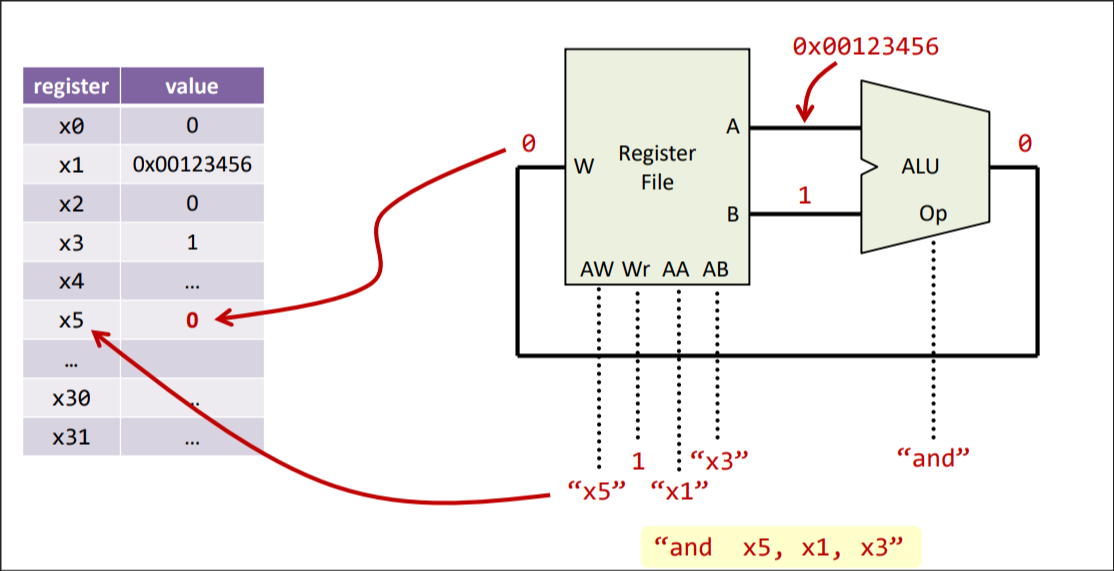
\includegraphics[scale=0.2]{screenshots/2025-10-11_3.png}
\end{center}
\subsubsection{The five classic components of a computer}
For an every day computer you need four other components other than the control components, you need to have a memory to store data (bigger than 32 word registers), you need to take input from the outside worlds (Internet, bluetooth, a keyboard, mouse ...) and also output something to the outside word.  On top of that, you need all of that to communicate $\implies$ you need a data path.
\begin{center}
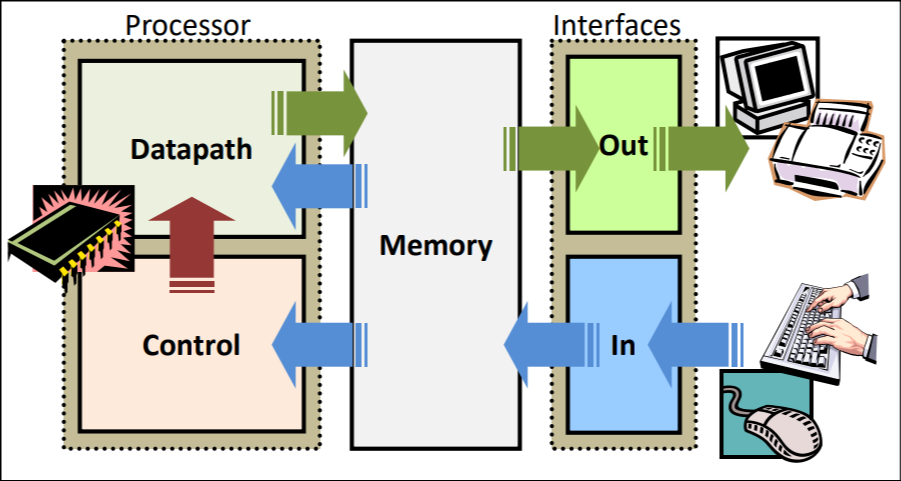
\includegraphics[scale=0.3]{screenshots/2025-10-11_4.png}
\end{center}
Okay, we have memory, we have input output and a place to compute everything, but what do we need to compute? Where is the program that is being executed? At the moment we have a place for the data but not for our program so how do we do it? \\ 
We store the program in the same memory than the one for the data. This is called a \textit{Unified Architecture} (On the other hand, an architecture that have two seperates memory, one for the instruction and one for the data is called a \textit{Harvard Architecture}). This is a \textbf{Key concept to computer science}, our instruction (therefore program) are represented as numbers (juste like data).
\begin{center}
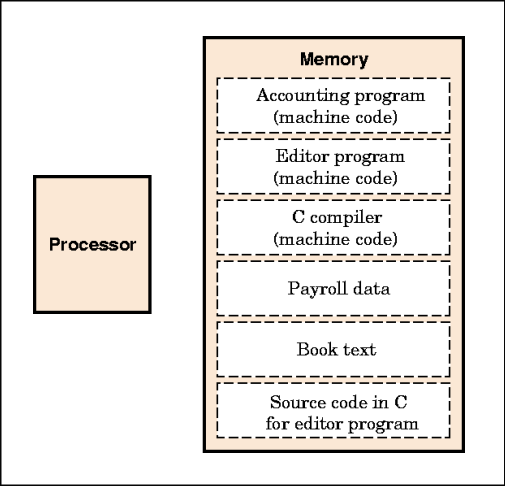
\includegraphics[scale=0.3]{screenshots/2025-10-11_5.png}
\end{center}
   Now a good question to have is: how to decode and encode those instructions and in the mean time, also what makes a good encoding? \\
A good encoding would be one that allows us two minimize the ressource in hardware and also is the fastest. This is where \texttt{RISC-V} comes in the play!! \texttt{RISC-V} is an instruction set architecture as like many others for instance x86, x64 for the most famous and used one.\\ 
The difference between assembly language and high-level language is in the "\textit{translation}", for the assembly language, we use an \important{assembler}, for a high-level language (a compiled one), we use a \important{compiler}:
\begin{itemize}
	\item Assembler can easily translate from code to binary code (this is what the instruction set tells us to do). All we need to do is the look up in the table and translate 
	\item A compiler on the other hand cannot look up in a table, it has to translate the code into Assembly code to be translated, but compiled the code into Assembly is a very hard thing to do, you have to find the best way or at least, try to find the best way to say the same thing but in assembly.
\end{itemize}


